\documentclass[12pt]{article}
\usepackage{sbc-template}
\usepackage{graphicx,url}
\usepackage[brazil]{babel}   

     
\sloppy
\title{Relatório: AI Creates Near Perfect Images Of People, Dogs and More}

\author{
    Romário Da S. Ferreira\inst{1},
    Marcos Yuri \inst{2}
}

\address{ Departamento Computação \\
        Universidade Tecnologica Federal do Paraná (UTFPR) 
        -- Medianeira, PR -- Brazil
        \email{{romario@alunos.utfpr.edu.br}, {marcosyuri.fsz@gmail.com} }
    }

\begin{document} 

\maketitle

\begin{abstract}
    Este relatório tem com objetivo descrever o estudo realizado no artigo
    AI Creates Near Perfect Images Of People, Dogs and More disponibilizado no canal Two Minutes Papers.
\end{abstract}
     
\begin{resumo} 
  This article aims to describe the study conducted in the article AI creates near-perfect images of people, dogs and more available on the Two Minute Documents channel.
\end{resumo}


% \section{General Information}
% 
% All full papers and posters (short papers) submitted to some SBC conference,
% including any supporting documents, should be written in English or in
% Portuguese. The format paper should be A4 with single column, 3.5 cm for upper
% margin, 2.5 cm for bottom margin and 3.0 cm for lateral margins, without
% headers or footers. The main font must be Times, 12 point nominal size, with 6
% points of space before each paragraph. Page numbers must be suppressed.
% 
% Full papers must respect the page limits defined by the conference.
% Conferences that publish just abstracts ask for \textbf{one}-page texts.
% 
\section{Introdução} \label{sec:firstpage}

%vou começar aqui 
O foco deste trabalho é analisar o \textit{Paper} "Generating Diverse High-Fidelity Images
with VQ-VAE-2" que na lingua portuguesa significa "Gerando imagens diversas de alta fidelidade utilizando VQ-VAE-2". O intuito do trabalho é gerar imagens de alta qualidade de uma grande variedade de classes, ou seja, animais, alimentos entre outros.. que sejam difíceis de analisar sua autenticidade sem que seja feita uma minuciosa análise.

O modelo de arquitetura que está descrito no \textit{Paper} utiliza a categoria de rede neural chamada Redes Generativas Adversarias (GANs). Resumindo as GANs são modelos de arquitetura em que duas redes com funções diferentes, sendo uma "generativa" que tem como o objetivo gerar amostras semelhantes a um certo conjunto de dados, enquanto a outra rede "discriminatória" avalia se as amostras geradas são verdadeiras ou falsas.

No \textit{Paper} também é descrito uma técnica de auto-codificação chamada Vector Quantized Variational AutoEncoder (VQ-VAE). O modelo VQ-VAE-2 é capaz de criar representações das instâncias do \textit{dataset} 30x menores com uma pequena perda de qualidade após a reconstrução. Além disso o \textit{encoder} e o \textit{decoder} é máis rápido e simples que o VQ-VAE original, o que possibilita a geração de imagens de alta qualidade.


\section{VQ-VAE}

O modelo do VQ-VAE é composto pelo \textit{encoder} e o \textit{decoder}, e o seu funcionamento pode ser descrito na Formula 1 

\begin{equation}
     Quantize(E(x)) = e_{k} where k = arg min_{j} || E(x) - e_{j}||
     \label{eq:saida-neuronio}
\end{equation}

Na etapa de \textit{encoder} é uma função não linear para o mapeamento do espaço $x$, para o vetor $E(x)$. O vetor pode ser quantificado pela distância para os vetores da galeria $e_{1}..e_{k}$, e cada vetor $E(x)$ é substituído pelo \textit{index} do vetor mais próximo da galeria, e depois transmitido para o decoder. 

Após a compactação da entrada, o \textit{decoder} tenta reconstruir por uma função não linear o espaço original dos itens da galeria que foi mapeado pelo \textit{encoder}.O calculo do erro dessa etapa é descrita na Formula 2, sendo $E$ a função de \textit{encoder}, $D$ a função de \textit{decoder}, $sg$ a operação de parada do gradiente e $\beta$ o hiper parâmetro 
\textit{bias}.

\section{PixelCNN}

O PixelCNN é um modelo Autoregressor Generativo é utilizado depois d  que utiliza a imagem como entrada, e a saída uma distribuição de sub-pixels para cada pixel.

\begin{equation}
     L(x,D(e)) = ||x - D(e)||_{2}^{2} + ||sg[E(x)] - e||_{2}^{2} + \beta||sg[e] - E(x)||_{2}^{2} 
     \label{eq:saida-neuronio}
\end{equation}



\section{Sections and Paragraphs}

Section titles must be in boldface, 13pt, flush left. There should be an extra
12 pt of space before each title. Section numbering is optional. The first
paragraph of each section should not be indented, while the first lines of
subsequent paragraphs should be indented by 1.27 cm.

\subsection{Subsections}

The subsection titles must be in boldface, 12pt, flush left.

%\section{Figures and Captions}\label{sec:figs}
%
%
%Figure and table captions should be centered if less than one line
%(Figure~\ref{fig:exampleFig1}), otherwise justified and indented by 0.8cm on
%both margins, as shown in Figure~\ref{fig:exampleFig2}. The caption font must
%be Helvetica, 10 point, boldface, with 6 points of space before and after each
%caption.
%
%\begin{figure}[ht]
%\centering
%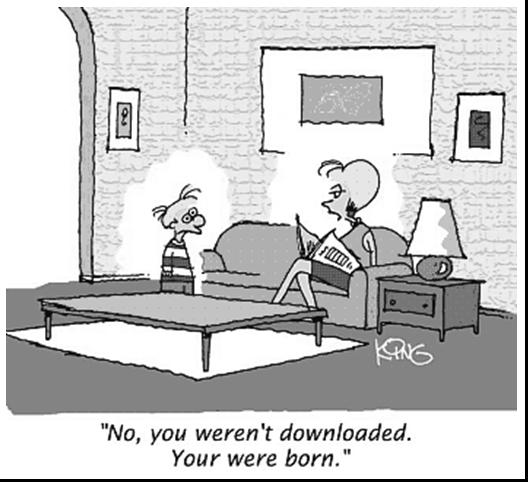
\includegraphics[width=.5\textwidth]{fig1.jpg}
%\caption{A typical figure}
%\label{fig:exampleFig1}
%\end{figure}
%
%\begin{figure}[ht]
%\centering
%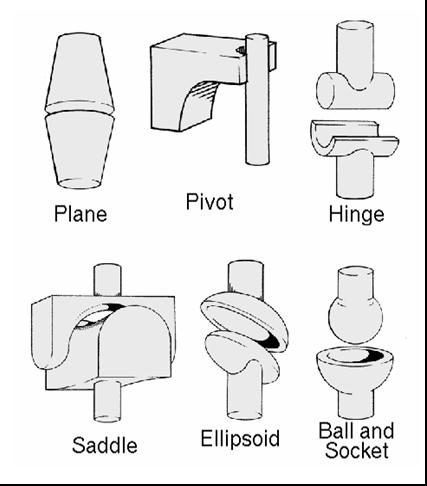
\includegraphics[width=.3\textwidth]{fig2.jpg}
%\caption{This figure is an example of a figure caption taking more than one
%  line and justified considering margins mentioned in Section~\ref{sec:figs}.}
%\label{fig:exampleFig2}
%\end{figure}
%
%In tables, try to avoid the use of colored or shaded backgrounds, and avoid
%thick, doubled, or unnecessary framing lines. When reporting empirical data,
%do not use more decimal digits than warranted by their precision and
%reproducibility. Table caption must be placed before the table (see Table 1)
%and the font used must also be Helvetica, 10 point, boldface, with 6 points of
%space before and after each caption.
%
%\begin{table}[ht]
%\centering
%\caption{Variables to be considered on the evaluation of interaction
%  techniques}
%\label{tab:exTable1}
%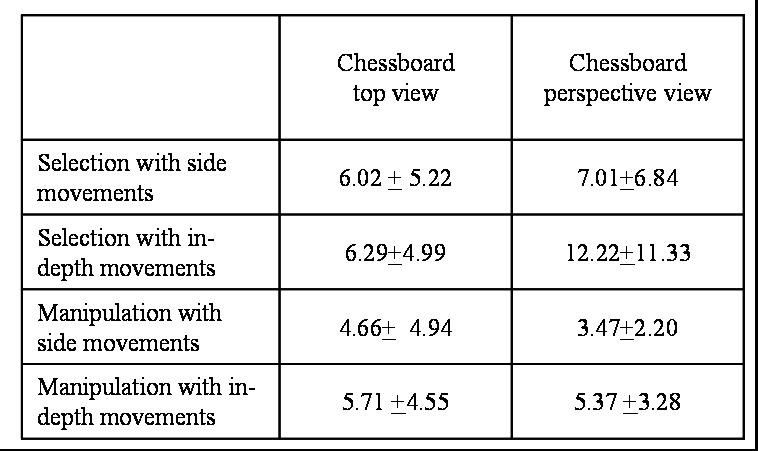
\includegraphics[width=.7\textwidth]{table.jpg}
%\end{table}
%

\section{Experimentos}
No Artigo em questão foi realizado uma avaliação e comparação de modelos generativos, ainda é vista como um desafio. Pois atualmente os modelos geram imagens que compensam a qualidade e diversidade de amostras. Desta forma foi apresentado resultados quantitativos e qualitativo do modelo treinado no imageNet 256x256. Visto que a qualidade da amostra foi realmente alta e nítida, assim várias classes representativas, como poderão ser visualizadas nas amostras condicionais de classes fornecidas no artigo em estudo. 

Em termos de diversidade, foi fornecido amostras do modelo ao lado de BigGan-deep, visto que o modelo GAN é de ultima geração. Assim pode-se visualizar as comparações lado a lado, VQ-VAE é responsavél e capaz de fornecer amostras de fidelidade comparável e com maior diversidade.

\subsection{Modelagem de imagens de rosto de alta resolução}
No estudo realizado, percebeu-se que para avaliar a eficácia da abordagem em várias escalas foi necessário capturar as dependências de alcance extremamente longo no conjunto de dados, assim foi treinado um modelo hierárquico de três níveis sobre o conjunto de dados FFHQ, o qual possuí resolução de 1024x1024.

Para efeito de entendimento, vale ressaltar que o conjunto de dados é composto por 70000 retratos humanos de alta qualidade possuindo diversidade farta de gênero, cor da pele, idade, poses e trajes.

Apesar da modelagem de faces ser normalmente considerada pouco dificultosa comparando-se com a imageNet, em tais resolução alta, pode-se existirem desafios de modelagem exclusivos que podem sondar modelos generativos de maneiras interessantes. Como exemplo, simetrias existentes nas faces requerem modelos capazes de obter dependências de longo alcance, pode-se observar o uso de um modelo com campo receptivo restrito no qual pode escolher cores 
possíveis para cada olho separadamente, assim como é apresentado no artigo, tal modelo pode perder a forte correlação entre os dois olhos que estão a centenas de pixels de distância um do outro, assim gerando amostras com cores de olhos contraditorias.
\subsection{Avaliação Quantitativa}
    É apresentado no artigo os resultados de avaliações quantitativas com base em diversas métricas, tais como objetivo de medir a qualidade e a diversidade de amostragens.

\subsubsection{Probabilidade de log negativo e erro de reconstrução}
As principais motivações para o uso de modelos generativos são baseados de acordo com o artigo, em probabilidade, no qual a probabilidade negativa de LOG nos conjuntos de teste e no treinamento fornecem uma medida objetiva para realiar a generalização e permite-nos monitorar o ajuste excecivo. 

Vale ressaltar que no é apresetado e enfantizado que outras métricas de desempenho são comumentes usadsa, tais como o FID e o Inception Score, quais ignoram completamente questões da generalização em um modelo que simplismente memoriza os dados de treinamento poderá obter uma pontuação perfeita em todas as outras métricas apilcadas. 

Tais métricas são baseadas são baseadas na amostragem e fornecem simplismente o proxy para viabilizar a qualidade e diversidade de amostras, mas não aludem à generalização de imagens retidas.

Sendo assim vale ressaltar e relatar que foi possível verificar a observação feita no artigo, onde os valores de NLL são comparáveis aprenas entre os modelos anteriores que usam o mesmo codificado e decodificador VQ-VAE pré treinado.
\subsubsection{Precisão - Métrica de Rechamada}
\subsubsection{Precisão da classificação}

\subsection{Probabilidade de log negativo e erro de reconstrução}



\section{References}

Bibliographic references must be unambiguous and uniform.  We recommend giving
the author names references in brackets, e.g. \cite{knuth:84},
\cite{boulic:91}, and \cite{smith:99}.

The references must be listed using 12 point font size, with 6 points of space
before each reference. The first line of each reference should not be
indented, while the subsequent should be indented by 0.5 cm.

\bibliographystyle{sbc}
\bibliography{sbc-template}

\end{document}
